%!TEX root = main.tex
  \section{Methods\label{sec:methods}}
  %to understand how VQSs can be used in scientific data analysis
  Via interviews and contextual \rchange{inquiry} in participants' normal work environments, we first identified the needs and challenges in participants' existing data analysis workflows. Given these challenges, we collaboratively designed VQS functionalities by engaging with experts from three different domains \cut{in the process of participatory design}\rchange{throughout the design process}, leading to a final prototype \zvpp. At the end of the \cut{design study}\rchange{co-design phase}, we conducted an evaluation study to understand how VQSs are used in the real-world analytical workflows. We will now describe the study procedure in more detail.
  %\subsection{Phase I: Contextual Inquiry and Participatory Design}
  \subsection{\rchange{Phase I: Contextual Inquiry \& Collaborative Prototyping}}
  \par We recruited participants by reaching out to research groups who have experienced challenges in data exploration, via email and word-of-mouth. Based on early conversations with analysts from 12 different potential application areas, we narrowed down to three use cases in astronomy, genetics, and material science for our design study, chosen based on their suitability for VQSs as well as diversity in use cases. Six scientists \cut{(1 female, 5 male), with an average of more than 6 years of}\rchange{, with extensive} research experience in their respective fields, participated in the design process. \cut{Via interviews and contextual inquiries,}\rchange{We interviewed participants to learn about their dataset and research questions, shadowed participants in performing their existing analysis workflows, and subsequently discussed the needs and challenges of their use cases. The interviews were semi-structured and focused on how the analytical tasks in their existing workflows relate to the scientific questions they were interested in.} We discuss these findings in Section~\ref{sec:participantdatasets}.% Our semi-structured interviews were loosely based on follow-ups on domain-specific details regarding their existing workflow (stemming from the early conversations), as well as were based on some preliminary understanding of each domain a set of task inclusion criteria for the types of tasks that we ---- in contextual inquiry. In particular, we focussed on studying how these analytic tasks relate to the scientific questions they were interested in.
  %based on each participant's existing analysis workflow
  %\par For the participatory design study, we built on an existing VQS, \zv~\cite{Siddiqui2017,Siddiqui2017VLDB}, that allowed users to sketch a pattern or drag-and-drop an existing visualization as a query, with the system returning visualizations that had the closest Euclidean distance to the queried pattern. We chose to build on top of \zv, since it was open-source, extensible, and included features beyond pattern and match specification typically found in existing systems (as compared in Table~\ref{table:relatedwork}) and described in Section~\ref{sec:sensemaking}. Past research on participatory design has found that the use of functional prototypes is a common and effective way of engaging with participants and providing a starting point for participatory design~\cite{Ciolfi2016}. Our motivation for providing a functional prototype at the beginning of the participatory design sessions was to showcase capabilities of VQSs. Since our participants were not aware of the existence of VQSs, let alone using them in their workflows, they would not have been able to imagine use cases for VQS without a starting point.%VQSs are not common in the existing workflows of these scientists, participants may not be
  %the participatory design study
  \par For \rchange{iterative prototyping}, we built on top of an existing open-source VQS, \zv~\cite{Siddiqui2017,Siddiqui2017VLDB}, to create a functional prototype \rchange{to showcase the capabilities of \rchange{VQSs}. The use of functional prototypes is a common and effective way of engaging with participants, by providing a starting point for \cut{participatory}\rchange{collaborative design}~\cite{Ciolfi2016}}. \cut{During participatory design, }\rchange{We} collaborated with each team closely with \cut{an average of}\rchange{approximately} two 1-hour-long meetings per month, where we learned \rchange{more} about their datasets, objectives, and what additional VQS functionalities could help address their research questions. \cut{Since some of the essential features that were crucial for effective exploration were lacking in \zv and still under development in the new version of our VQS, \zvpp, we did not provide a deployed prototype for participants to actively use on their own during the design phase.} \rchange{During these meetings, we iterated on the design of features in our prototype and relevant capabilities from the prototype were demonstrated to the participants.} \rchange{As ``\textit{simulated future work situations}'' are commonly used in cooperative prototyping~\cite{Grnbak1991}}, participants also had the opportunity to interact with the \cut{low-fidelity} prototype through the help of a guided facilitator. \rchange{Through these excercises,} we elicited feedback from participants on how the VQS could better support their scientific goals and identified and incorporated several crucial capabilities into \zvpp, described more in Section~\ref{sec:pd_findings}.
  %\par Since some of the essential features that were crucial for effective exploration were lacking in \zv and still under development in the new version of our VQS, \zvpp, we did not provide a deployed prototype for participants to actively use on their own during the participatory design period. Instead, as we iterated on the design of these features, relevant capabilities from intermediate versions of \zvpp were demonstrated to the participants. \rchange{As ``\textit{simulated future work situations}'' are prevalent in cooperative prototyping~\cite{Grnbak1991}}, participants also had the opportunity to interact with the \cut{low-fidelity} prototype through the help of a guided facilitator. %Such use of ``\textit{simulated future work situation}'' is common in cooperative prototyping when the real use of the prototype is not feasible~\cite{Grnbak1991}.  During this process, we elicited feedback from participants on how the VQS could better support their scientific goals. 
  \cut{A summary timeline of our collaboration with participants over a year can be found in Figure \ref{timeline} in Appendix \ref{apdx:pdartifact}.} %During these sessions, we discussed and iterated on the design of additional features for \zvpp.
  %Participants provided datasets they were exploring from their domain, whereby they had a vested interest in using a VQS to address their own research questions.
  %into the new version of our VQS,
  %Through this process, we identified and incorporated several crucial capabilities into \zvpp.\cut{, as listed in Table~\ref{bigfeaturetable}.} % , described more in Section~\ref{sec:pd_findings}.
  \begin{table}[hb!]
    \centering
    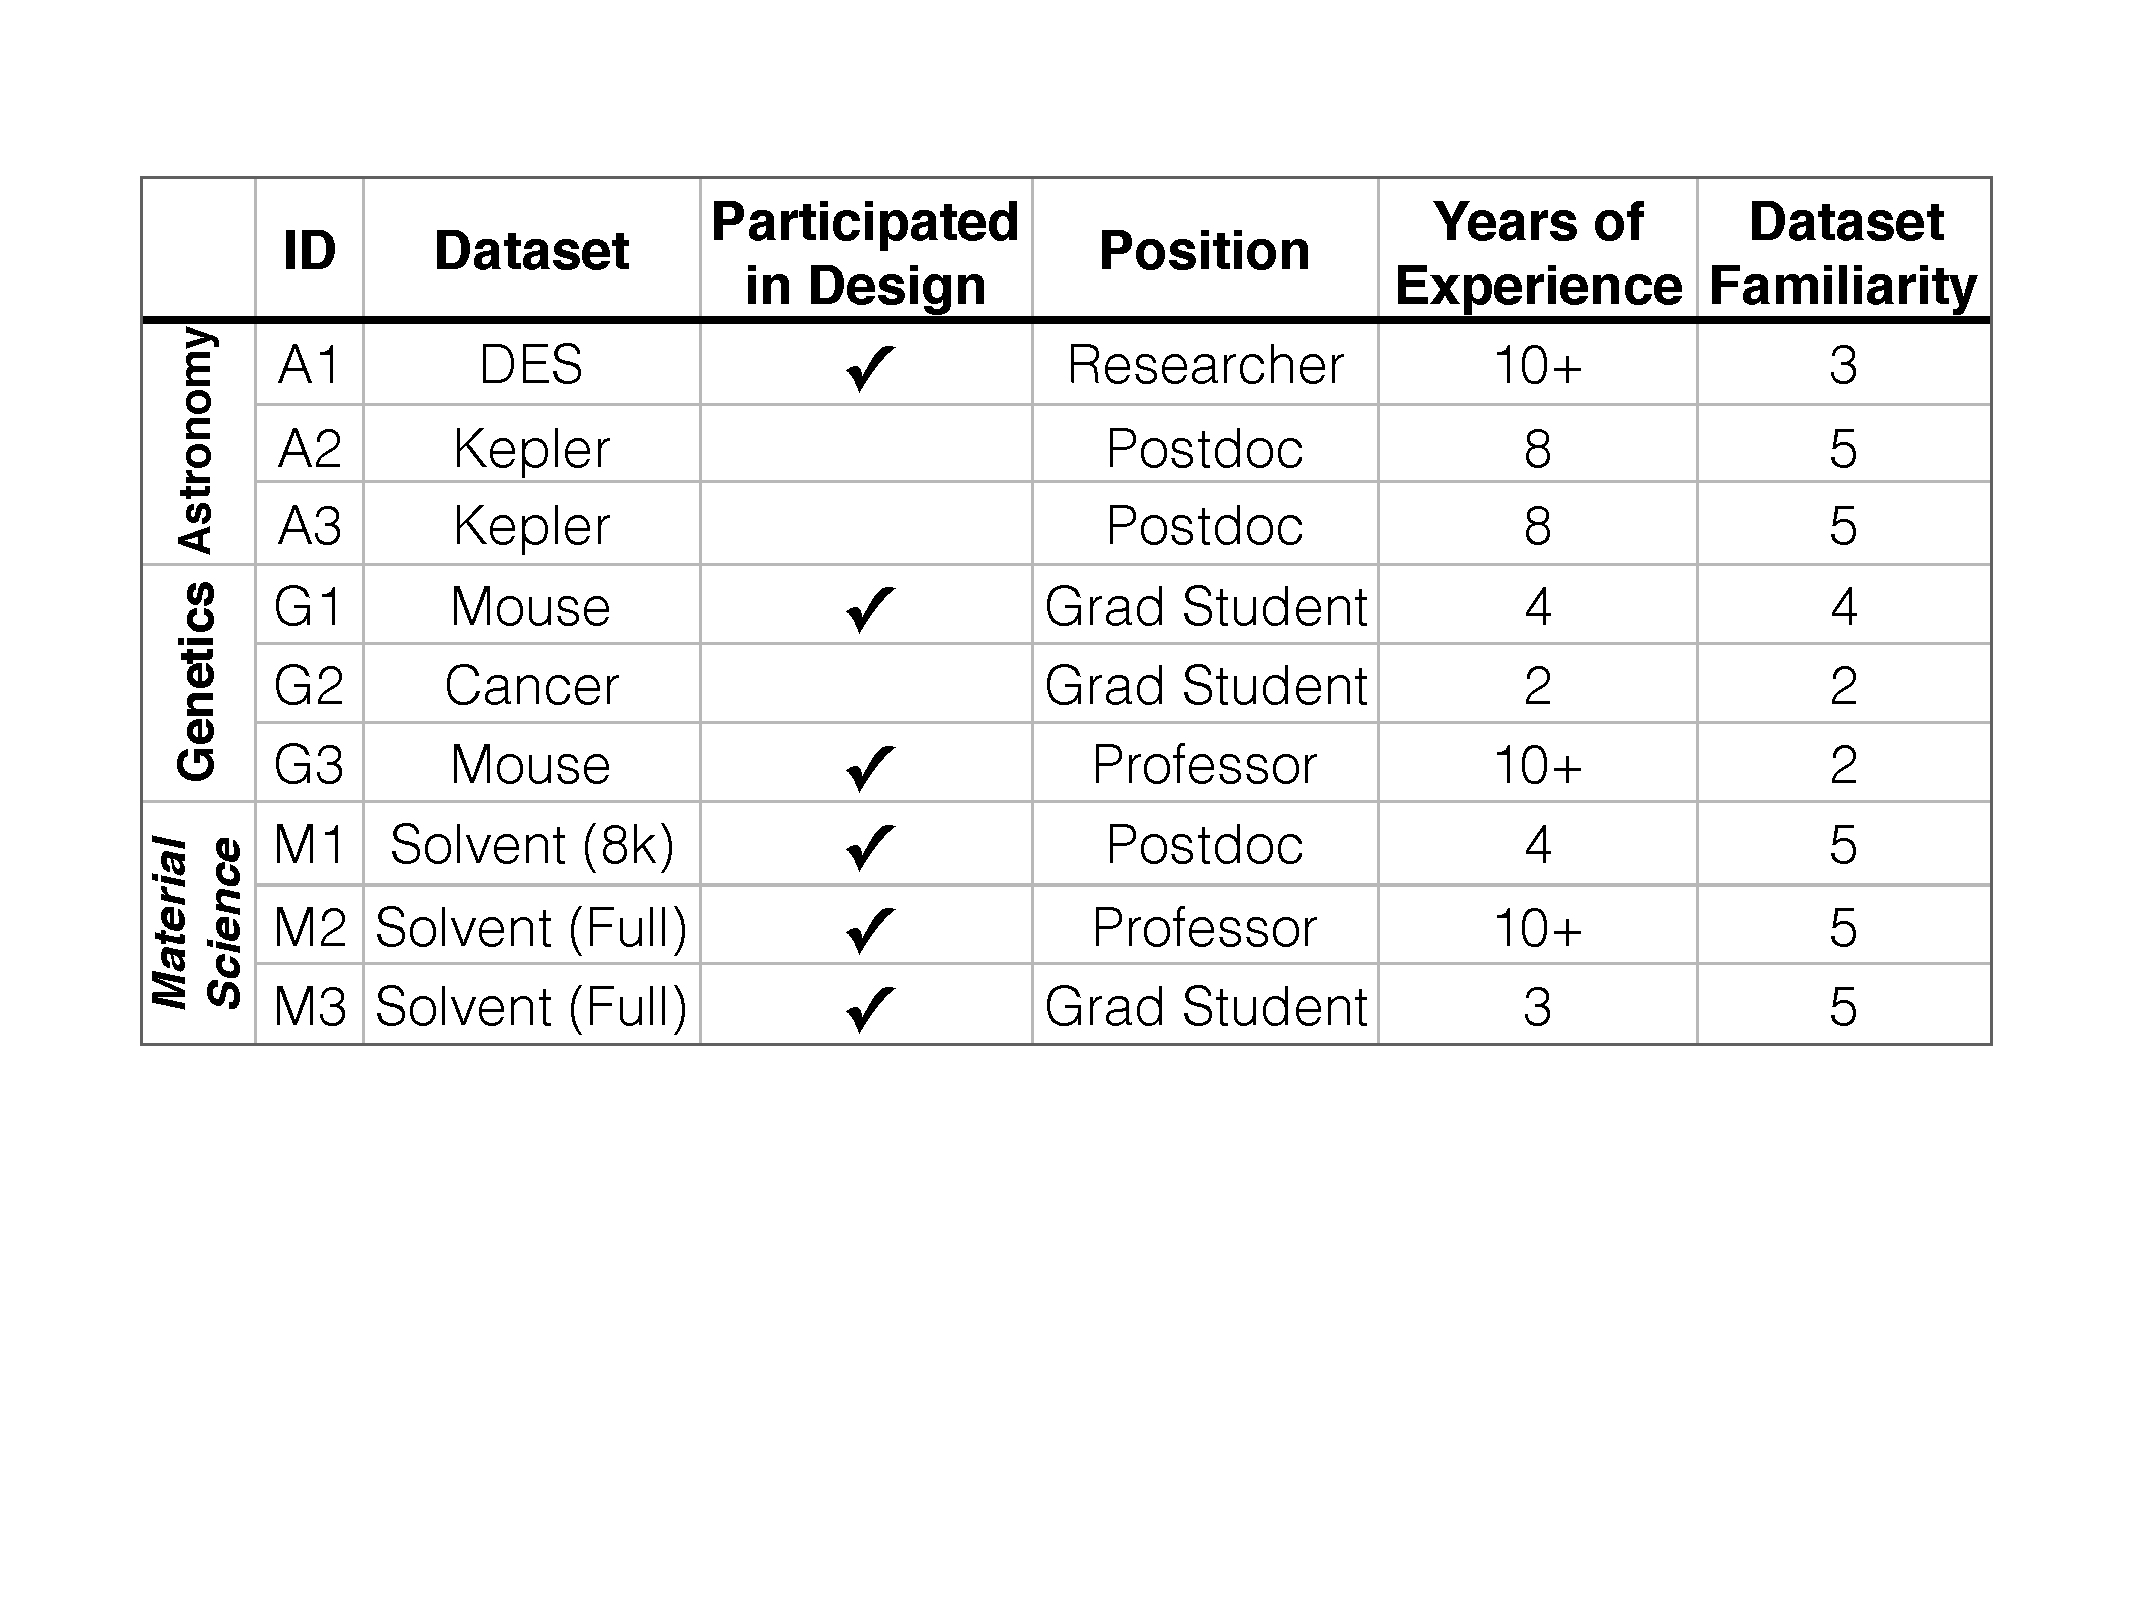
\includegraphics[width=0.9\linewidth]{figures/participant_info.pdf}
    \caption{Participant information. The Likert scale used for dataset familiarity ranges from 1 (not familiar) to 5 (extremely familiar).}
    \label{participants}
    \vspace*{-10pt}
  \end{table}
  % \subsection{Phase II: Evaluation Study}
  \subsection{\rchange{Phase II: Qualitative Grounded Evaluation Study}}
  % \par Visualization systems are often evaluated using controlled studies that measure the user's performance against an existing visualization baseline~\cite{Plaisant2004}. Techniques such as artificially inserting ``insights'' or setting predefined tasks for example datasets work well for objective tasks, \techreport{such as debugging data errors~\cite{kandel2011wrangler,Patel2010},} but they are unsuitable for trying to learn about the types of real-world queries users may want to pose on VQSs. %Due to the unrealistic nature of controlled studies, many have proposed using a more multi-faceted, ethnographic approach to understand how analysts perform visual data analysis and reasoning~\cite{Plaisant2004,lam2012empirical,shneiderman2006strategies,munzner2009nested,Sedlmair2012}.
  %In order to make the evaluation more realistic, we invited p
  At the end of our \rchange{design study}, we performed a qualitative evaluation to study how analysts interact with different VQS components in practice. Participants used datasets that they have a vested interest in exploring to address unanswered research questions (a total of six different datasets across nine participants). As shown in Table~\ref{participants}, the evaluation study participants included the six scientists from \rchange{the design phase}, along with three additional ``blank-slate'' participants who had never encountered \zvpp before. The use of all or a subset of the project stakeholders as evaluation participants is typical in participatory design~\cite{Bossen2016}. While the small sample size of participants may be viewed as a limitation, as echoed in prior work\cite{Batch2018,Mclachlan2008}, this is a pervading challenge when recruiting domain-experts\cut{, whose specific expertise and skills are rare and have limited time due to their workplace demands relative to the general population}. Nevertheless, as Sedlmair et al.~\cite{Sedlmair2012} argue, even studies with a small group of domain experts involved are invaluable for understanding expert needs. % Despite these challenges, ----- is still invaluable to ----- (CITE).
  %\dor{Addressing Aditya's comments, we can't exactly say that most other PD work involves significantly fewer participants. For example, LiveRAC involved 14 participants in 3 groups; Batch and Elmqvist had  8 participants. So our study is about typical in size.}
  %As detailed in Table~\ref{participants}, the nine participants brought a total of six different datasets to the study. 
  %and ---- to participate in studies
  %(e.g., stakeholders)
   %\cut{Since the participatory design subjects acted as informants and did not actively try out the system on their own, the evaluation study was the first time that all participants used \zvpp to explore their datasets.}
  %\ccut{While participatory design subjects actively provided feedback on \zvpp with their data, they only saw us demonstrating their requested features and explaining the system to them, rather than actively using the system on their own. So}
  % \dor{We could summarized the next two paragraph as simply participants engaged in talk-aloud excercise while exploring their datasets using \zvpp...Replacing everything until "The user study ended after ...". But if we are not short on space, we can keep the existing description.}
  \par Evaluation study participants were recruited from each of the three aforementioned research groups, as well as domain-specific mailing lists. Prior to the study, we asked potential participants to fill out a pre-study survey to determine eligibility. Eligibility criteria included: being an active researcher in the subject area with more than one year of experience, and having worked on a research project involving data of the same nature used in \rchange{the design phase}. \cut{None of the participants received monetary compensation for the study, as this is not a common practice for \rchange{collaborative} design with stakeholders~\cite{Ommen2016,McNally2017}.} \techreport{The research questions and objectives of the participants were diverse even among the same subject area. Examples included understanding gene expression profiles of breast cancer cells after a particular treatment and comparing common patterns among stars that exhibit planetary transits versus stars that do not.\techreport{from the Kepler space telescope\footnote{\url{www.nasa.gov/mission_pages/kepler/main/index.html}}.}}
  \par At the start of the \rchange{in-lab evaluation} study, participants were provided with an interactive walk-through of \zvpp and given approximately ten minutes for a guided exploration of a preloaded real-estate example dataset. \techreport{from Zillow \cite{zillow}. This dataset contained housing data for various cities, metropolitan areas, and states in the U.S. from 2004-15.}After familiarizing themselves with the tool, we loaded the participant's dataset and encouraged them to talk-aloud during data exploration, and use external tools or other resources as needed. If the participant was out of ideas\ccut{ for three minutes}, we suggested one of the main VQS functionalities\cut{\footnote{query by sketching, drag-and-drop, pattern loading, input equations, representative and outliers, narrow/ignore x-range options, filtering, data smoothing, creating dynamic classes,  data export}} that they had not yet used. If any of these operations were not applicable to their specific dataset, they were allowed to skip the operation after having considered it. The user study \rchange{lasted for about an hour and} ended after they covered all the main functionalities. After the study, we asked participants open-ended questions about their experience.% and lasted on average for 63 minutes.